In dem folgenden Kapitel sollen die Ergebnisse der Implementierungen ausgewertet und analysiert werden. Dafür wurden einige Kriterien ausgewählt und die Implementierungen und sonstige Quellen daraufhin untersucht und verglichen.

\section{Performance und Entwicklung}
Bei einigen Implementierung geht es auch stark um die Performance der entwickelten Anwendungen. Die Performance und einige andere Faktoren der Entwicklung sollen im folgenden etwas genauer unter anderem durch gemessene Werte analysiert werden.

\subsubsection{Dauer typischer Entwicklungsoperationen}
Wenn es um Entwicklungzeit und Fortschritt geht, dann ist oft auch ein Faktor, wie lange die App braucht um gebaut zu werden und wie lange es dauert um Änderungen in der App anzuzeigen. Oft muss bei der Entwicklung von Oberflächen einige Kleinigkeiten geändert und dann überprüft werden, ob die Änderung den gewünschten Effekt hatte. Deshalb sind vor allem kurze ladezeiten von Änderungen besonders wichtig.

Für diesen Test wurde die Dauer des erstmaligen Compilieren, die Dauer eines Neubauens auf Basis eines bestehenden Caches, die Dauer bis Layoutänderungen und bis Anwendungslogik geladen wurde, im Debug Modus durchgeführt. Es wurde außerdem die Compilierzeit im Release Modus aufgezeichnet.
Die Tests hierfür wurden jeweils fünf mal ausgeführt und dann am Ende ein Durchschnitt gebildet. Als Hardware wurde ein PC mit 32GB RAM und einer Ryzen 5 2600 6-Kern CPU genutzt. 
Die genauen Zahlen sind von der genutzten Hardware und der Projektgröße abhängig, geben aber einen Einblick ob hier einzelne Ansätze einen Vorteil haben. 

\begin{table}
\centering
\caption{Dauer typischer Entwicklungsoperationen in Sekunden}
\begin{tabular}{ |p{4cm}||p{3cm}|p{2cm}|p{2cm}|p{3cm}|p{3cm}| }
 \hline
 Funktion & Flutter-Hybrid & Flutter & Kotlin-Nativ & Kotlin-WebView \\
 \hline
 Build Zeit Release       &   59,2&   54,22& 40,92& 22,42\\
  \hline
 Build Zeit Debug  & 33,78& 28,76& 20,2& 20,19\\
  \hline
 Erneuter Build mit Cache & 8,8& 8,36& 3,36& 3,21\\
  \hline
 Neuladen nach Layoutänderg & 0,59& 0,6& 2,59& 2,64\\
  \hline
 Neuladen nach Logikänderung & 0,626& 0,622& 3,18& 2,63\\
  \hline
\end{tabular}
\label{tab:evaluations_build_time}
\end{table}

Bei der Analyse der Daten fällt auf, dass grundsätzlich bei der Build Zeit die Flutter Apps schlechter abschließen. Sowohl beim Erstellen einer Release oder auch Debug \ac{APK} sind die Kotlin Applikationen schneller. Bei der Debug \ac{APK} ist der Unterschied jedoch deutlich geringer und selbst die Kotlin-WebView App benötigt in etwa gleich lang, wie die native Kotlin Implementierung. Beim Compilieren einer Release App scheint es daher tatsächlich mehr um den Umfang der Applikation zu gehen, als bei der Debug Version.

Der auffälligste Unterschied ist jedoch die Neuladezeit nach einer Änderung im Quellcode. Denn Flutter schneidet dank des HotReload Features hier deutlich besser ab und benötigt somit gerade mal 1/5 der Zeit die die mit Koltin implementierten Applikationen benötigen. Dazu kommt, dass beim Neustarten bei Android, die Applikation vom Startbildschirm neustartet, während Flutter nur die Änderungen in die aktuelle Seite lädt und diese neustartet. Dadurch muss nicht erst wieder zu der aktuell entwickelten Stelle zurückgekehrt werden. So wrid etwa die Farbe eines Textes im Fluttercode geändert und innerhalb von 600ms wird die Änderung angezeigt. So wird nicht nur Zeit gesparrt, sondern es kann sich auch besser darauf konzentriert werden, eine ordentliche Nutzeroberfläche zu entwickeln.

\subsubsection{Performance}

\begin{table}
\centering
\caption{Performancemessung der verschiedenen Applikationen }
\begin{tabular}{ |p{4cm}||p{3cm}|p{2cm}|p{2cm}|p{2cm}|p{2cm}| }
 \hline
 Parameter & Flutter-Hybrid & Flutter & Kotlin-Nativ & Kotlin-WebView \\
 \hline
 Durchschnittliche CPU-Auslastung       &   2,54\%&   1,96\%& 0,9\%& 1,8\%\\
  \hline
 Maximale CPU- Auslastung  & 9,8\%& 6,4\%& 3,6\%& 7,4\%\\
  \hline
 Durchschnittliche RAM-Auslastung & 215,38 MB& 150,68MB& 86,74MB& 107,68MB\\
  \hline
 Maximale RAM- Auslastung & 238MB& 175,46MB& 100,64MB& 117,06MB\\
  \hline
 App-Größe & 8,6MB& 8,4MB& 5,2MB& 4,4MB\\
  \hline
 Maximale Startzeit & 532ms& 452ms& 263ms& 486,6ms\\
 \hline
 Durchschnittliche Renderzeit &8,68ms& 5,12ms& 9,04& 21,88ms\\
 \hline
\end{tabular}
\label{tab:evaluations_performance}
\end{table}

In Tabelle \ref{tab:evaluations_performance} sind die Ergebnisse der Performance-Messungen zu sehen, die an den beschriebenen Implementierungen durchgeführt wurden.
Die Messungen wurden mit dem Programm Apptim durchgeführt. Dies zeichnet die Performance von Apps während der Nutzung einer App auf. Die Tests wurden auf einem Google Pixel 5 durchgeführt mit Android Level 12 oder auch API Level 31. Es hat dabei 8GB DDR4-Ram und einer 8-Kern-CPU, die mit 6x1,8GHz, 1x2,2GHz und 1x2,4GHz getaktet sind.
Der Test wurde dabei für jede Implementierung 5 mal wiederholt und aus den Ergebnissen dann ein Durchschnittswert gebildet. Die Apps wurden nach jeder Nutzung zurückgesetzt und alle anderen Apps wurden während der Tests beendet. Die Apps waren dafür jeweils als Release-Version installiert, so dass die Apps bei bester Leistung wie auch bei einem Endbenutzer laufen würden.
Renderzeit entspricht der Zeit, die gebraucht werden, bis die Änderungen geziechnet wurden und als Bild angezeigt werden können

Hierbei ist erkennbar, dass die native Android App insgesamt die schnellste ist, während die Hybride Flutter App die am schlechtesten performende. Die schnellste Renderzeit hatten die Flutter-Applikationen, während die Auslastung des Rams bei den Android Applikationen deutlich geringer war. Überraschend zu sehen ist, dass die WebView Applikation mehr Ressourcen verbraucht als die nativ implementierte, obwohl sie lediglich einen WebContainer bauen muss. was außerdem auffällt, ist dass Flutter Applikationen etwa zwei mal so groß sind als die nativen. Eine weitere Sache ist, dass die die Android Apps und die reine Flutter App sehr vergleichbar sind, während die Hybride Flutter App in fast jeder Kategorie doppelt so viele Ressourcen verbraucht hat, wie die native Android Anwendungen.

Was festhalten werden kann, ist, dass eine Flutter App zwar in der Performanz etwas den nativen geschriebenen Applikationen hinterherhängt, jedoch der Unterschied nicht derart groß ist, als dass er eine große Rolle spielen würde. Was jedoch auffält ist das die hybride Flutter App Performance technisch deutlich schlechter abschneidet als die native.  

Biorn Hansen et al\cite{BirnHansen.2020} sagen in ihrer Auswertung, dass sie einen deutlichen Anstieg bei Datenbankbenutzung sehen konnten. Deshalb wurde bei der Flutter App und der nativen Android App  jeweils eine Datenbankimplementierung nach der Dokumentation der einzelnen Plattformen eingefügt. Daraufhin wurden beide Apps wieder wie oben beschrieben getestet und am Ende der Anstieg in den einzelnen eine Applikationen ausgewertet und in Tabelle \ref{tab:evaluations_performance_Overhead_database} zusammengetragen.

Auffällig ist, dass die CPU auslastung bei beiden gleichmäßig ansteigt, während bei der Nativen die RAM Nutzung deutlich mehr ansteigt, als bei der Flutter. Wenn Tabelle \ref{tab:evaluations_performance} miteinbezogen wird, nutzt die native App damit immer noch weniger Ram als die normale Flutter, da diese bereits ohne Datenbank eine recht hohe RAM Nutzung hat. Bei der App Startzeit ist die Flutter App, die nochmal 60 ms mehr länger braucht als die Android und somit nun 36\% langsamer ist als die Native. Bei der Renderzeit zeigt sich weiterhin die stärke von Flutter, da hier ein deutlich geringerer Anstieg zu verzeichnen ist.

\begin{table}
\centering
\caption{Unterschied bei Implementierung mit zusätzlicher Datenbankimplementierung}
\begin{tabular}{ |p{7cm}||wc{3.5cm}|wc{3.5cm}|}
 \hline
 Parameter & Flutter &  Kotlin-Nativ \\
 \hline
 Durchschnittliche CPU-Auslastung       &  0,44\%&   0,26\%\\
  \hline
 Maximale CPU-Auslastung  & 2,2\%& 2,6\%\\
  \hline
 Durchschnittliche RAM-Auslastung & 5,64 MB& 18,04MB\\
  \hline
 Maximale RAM-Auslastung & 4,98MB& 39,64MB\\
  \hline
 App-Größe & 0,1MB& 0,1MB\\
  \hline
 Maximale Startzeit & 221ms& 162,6ms\\
 \hline
 Durchschnittliche Renderzeit &0,82ms& 4,68ms\\
 \hline
\end{tabular}
\label{tab:evaluations_performance_Overhead_database}
\end{table}

Grundsätzlich kann festgehalten werden, dass native Entwicklungen meistens die beste Performance haben werden, Jedoch ist mit Flutter ein Framework auf den Markt gekommen, das dies in Frage stellt. Denn Flutter ist wie bereits erwähnt ein Framework, dass den geschriebenen Dart-Code in Nativen Code umwandelt. Es hat sich außerdem zum Ziel gesetzt, möglichst performant zu sein. Eine Untersuchung von Biørn-Hansen et al hat ergeben, das Nativ zwar immer noch am performantesten ist, Flutter in einigen Kategorien auch noch etwas hinten an ist, jedoch dieser Unterschied nicht besonders groß ist  \cite{BirnHansen.2020}.

Eine andere Untersuchung zeigte, dass  es darauf ankommt, was man macht\TODO{Hier fehlt noch was}

\subsubsection{Debugging/Testing}
Bei Debugging und Testing stehen zumindest in unseren Testfällen die Apps beim Applikationscode in keinem Teil nach. Bei allen kann man sowohl Breakpoints als auch Konsolenausgaben veranlassen. Es können auch für alle Arten Tests geschrieben werden.

Bei den hybriden Ansätzen ist die Debug und Test Möglichkeiten  durch die Web-Implementierung allerdings teils stark eingeschränkt. Wenn etwa wie in diesem Fall die Web-Implementierung nicht innerhalb der Applikation sonder auf einem externen Server läuft, müssen die beiden Teile getrennt betrachtet werden. Dies ist auch mit allen Frameworks möglich, bedeutet jedoch einen erhöhten Aufwand und erschwert die Fehlerfindung mitunter.

\section{Community}
Die Entwickler Community ist ein wichtiger Faktor für die Wahl eines Frameworks. Wenn es keine Community gibt, wird es schwer Entwickler oder auch Lösungen für Probleme zu finden, ohne sie selber zu entwickeln. Aber nicht nur Bibliotheken helfen dabei, schneller zu entwickeln sondern auch Frage-Antwort Communities wie Stackoverflow\footnote{https://stackoverflow.com/}.  Die genauen Zahlen der Community-Größe oder die Populärität sind dabei nicht genau bestimmbar. Sie können jedoch anhand einiger Faktoren annähernd bestimmt werden, bzw. verglichen werden.

\subsubsection{Star-History}

Ein erster Anhaltspunkt ist die Sogenannte Star-Anzahl von Github-Repositorys. Es gibt an, wie viele Leute sich die Repositories mit einem Stern markiert haben, um über Neuerungen informiert zu werden. Es gibt also keine absolute Zahl wie viele Leute mit einem Framework oder Programmiersprache entwickeln, es zeigt jedoch ganz gut wie viel Interesse Leute an der Entwicklung dieser haben.

\begin{figure}[ht]
  \centering
  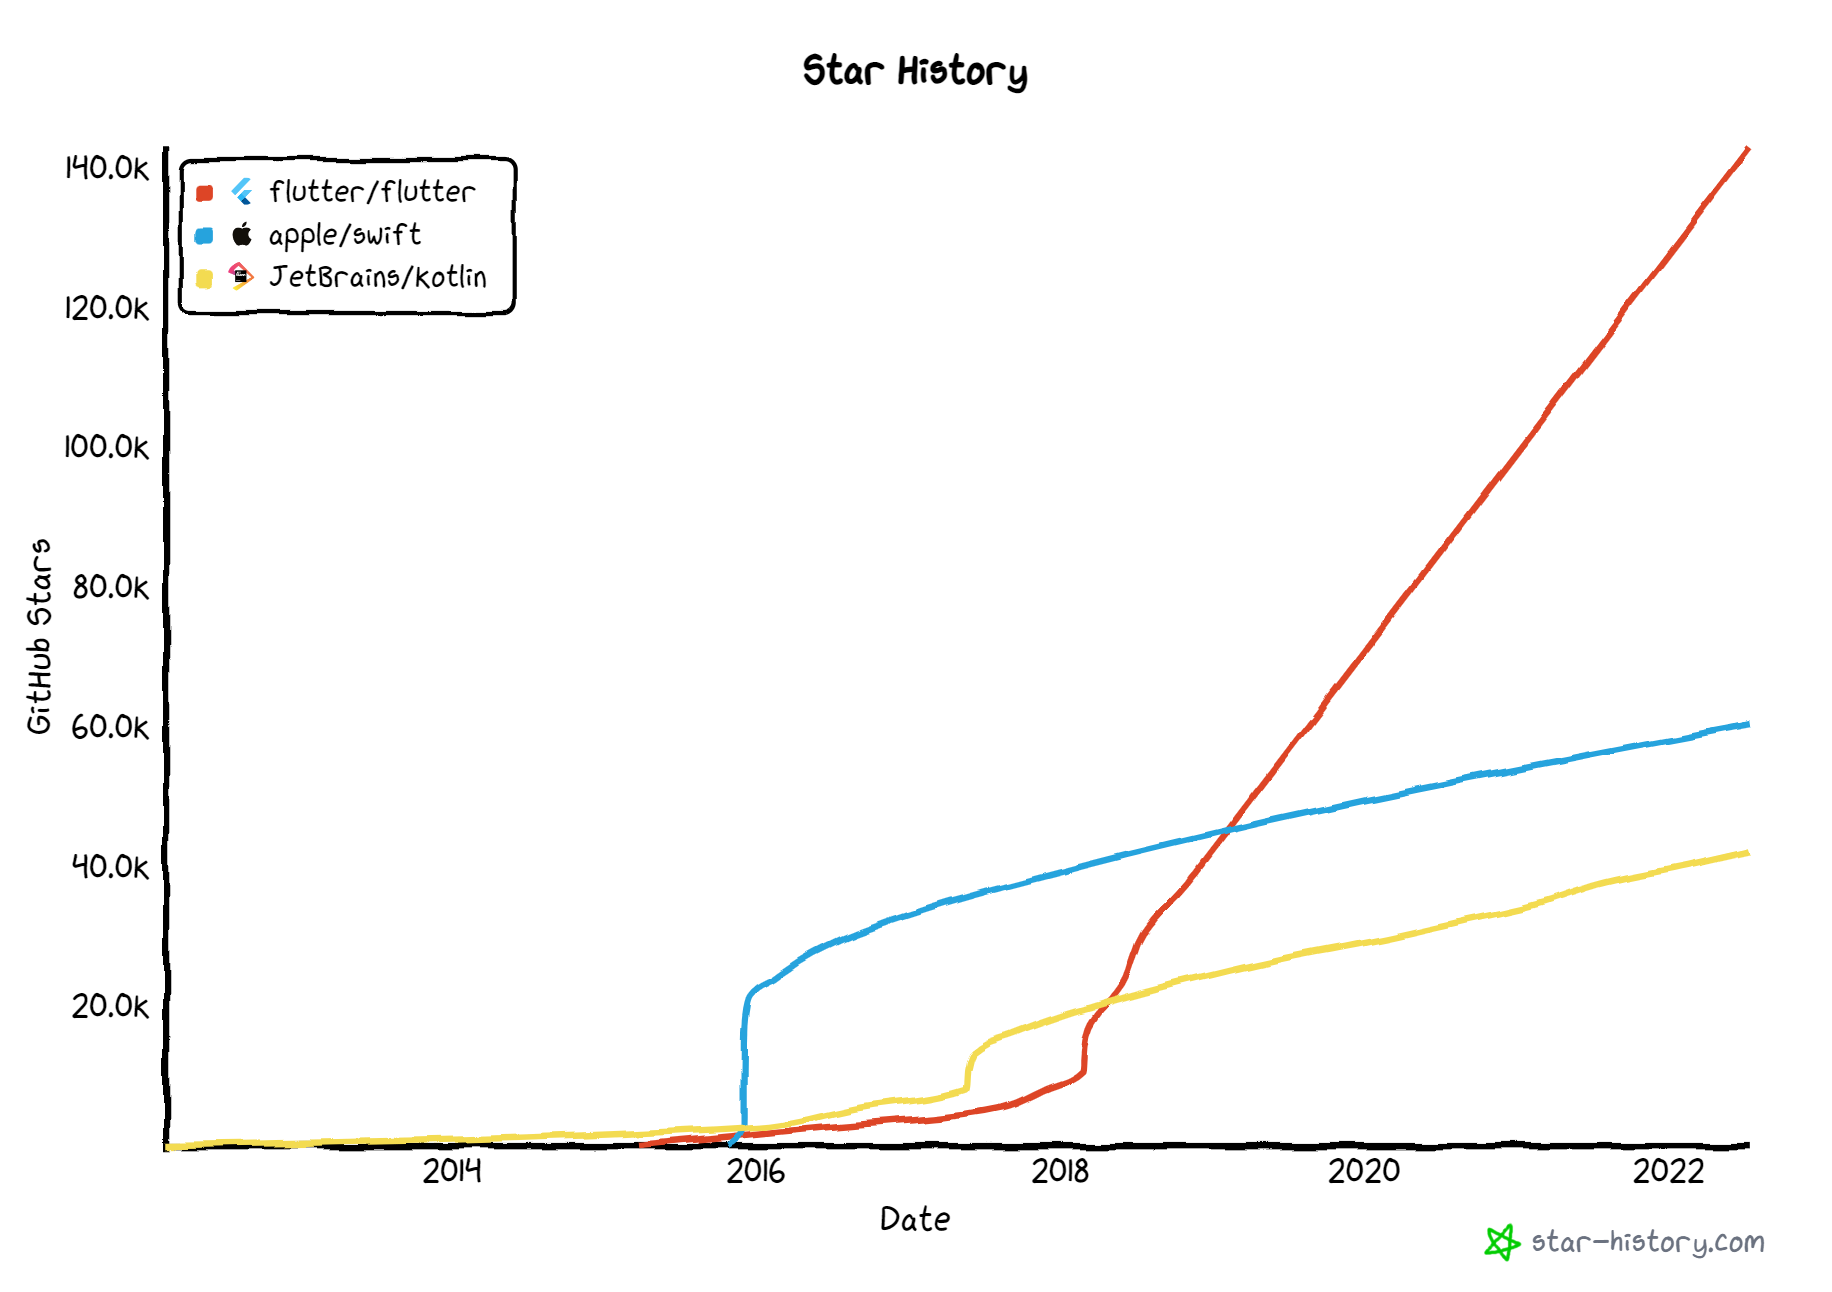
\includegraphics[height=7cm,keepaspectratio]{images/star-history_programming languages.png} 
  \caption[Zeitlicher Verlauf von Stars der Github-Repositorys von Swift, Kotlin und Flutter]{Zeitlicher Verlauf von Stars der Github-Repositorys von Swift, Kotlin und Flutter\protect\footnotemark }
  \label{fig:star_history}
\end{figure}
\footnotetext{https://star-history.com/\#flutter/flutter\&JetBrains/kotlin\&apple/swift\&Date}


Abbildung \ref{fig:star_history} zeigt ein mit Hilfe der GitHub-Api erstelltes Diagramm der Anzahl der Stars der Swift, Kotlin und Flutter Repositories im zeitlichen Verlauf. 
Besonders gut zu erkennen ist, wie stark das Interesse an Flutter ist. Nach der ersten Änkündigung 2018 und der darauf ersten veröffentlichten Version ist die Zahl der Interessierten innerhalb von 4 Jahren auf 140 000 angestiegen. Das Repository für Swift und Kotlin haben im gleichen Zeitraum gerade mal 20 000 Stars dazu erhalten. Dabei haben Swift und Flutter beide innerhalb des ersten Jahres nach Vorstellung etwa 30 000 Stars gemacht. Jedoch ist das Interesse an Swift danach abgeflacht und verläuft aktuell parallel zu Kotlin. Es zeigt also doch, dass das Interesse sehr hoch ist.

\subsubsection{Stackoverflow}
Ein weiterer Anhaltspunkt ist die Anzahl an gestellten Fragen auf Stackoverflow\footnote{https://stackoverflow.com/}. Stackoverflow ist für viele Entwickler ein guter Ort um Lösungen oder Code zu finden, um die aufgetretenen Probleme zu lösen. Stackoverflow kann durch Filterung etwa die Anzahl der Fragen ausgeben. Hierfür wurden die Anzahl der Fragen für Kotlin, Swift und Flutter der letzten 2 Jahre gesammelt. Dabei wurden auch eventuelle Überschneidungen herausgefiltert und es musste mindestens eine Antwort geben.

Für Kotlin sind es 105 082\footnote{Filter: [kotlin] or [android][kotlin] or [android]-[flutter]-[java] lastactive:2y.. is:question answers:1..}, für Swift 71 749\footnote{Filter: [swift] or [ios][swift] or [ios]-[flutter]-[objectivc] lastactive:2y.. is:question answers:1..} und bei Flutter 77,568\footnote{Filter:[flutter] or [dart] -[ubuntu] lastactive:2y.. is:question answers:1..}Fragen.

Flutter hat also scheinbar ebenfalls eine aktive Community die durchaus mit der von Kotlin und Apple mithalten kann. Hier muss jedoch eingeschrenkt werden, dass manche Fragen schon vor dem untersuchten Zeitraum gestellt wurden und deswegen eine Frage nicht in dem untersuchten Zeitraum erneut auftaucht. Da sowohl Kotlin als auch Swift bereits länger auf dem Markt sind, dürfte die Anzahl der Fragen die deshalb nicht gestellt wurden, höher sein als bei Flutter, jedoch kann trotzdem festgestelt werden, dass es hier dennoch genügend Leute vorhanden sind, um Hilfe bei Problemen zu erhalten.

\subsubsection{Dokumentation}
Ein weiterer wichtiger Faktor ist Dokumentation. Hierbei, haben sowohl Flutter als auch Kotlin eine umfangreiche und von den Entwicklern dauerhaft aktualisierte und erweiterte Dokumentationsseite. Wo jedoch Flutter einen Vorteil zu Kotlin hat, ist ein zentraler Ort\footnote{https://pub.dev/} wo man nach weiteren Plugins, Bibliotheken, Widgets und vielem mehr suchen kann. Hier sind nicht nur offizielle Flutter Repositorys verlinkt, sondern jeder aus der Community kann seine Plugins hier verlinken. Neben einem Punktesystem, dass diese bewertet, wie viele Richtlinien es einhält, wird außerdem angezeigt, für welche Plattformen das angezeigte Projekt funktioniert. So kann einfach nach den passenden Erweiterungen gesucht werden, ohne sich durch GitHub-Repositorys zu hangeln, um nach einer passenden Bibliothek zu suchen.

Die Dokumentation für die verschiedenen Ansätze ist allerdings etwas anders. So gelten alle bisherig getroffenen Aussagen vor allem für die native und Cross-Plattform Lösung, da hier die Frameworks und ihre Programmiersprachen dafür eingesetzt werden, wofür sie entwickelt wurden. Für die hybride beziehungsweise die Mix-Implementierung ist dies anders. So kann zwar die in der Regel gute Dokumentation für die gewählte Grundlagen und die Web Implementierung genutzt werden, jedoch ist eine Dokumentation für den genauen Ansatz selten oder nur begrenzt vorhanden. So gibt es etwa einige Tutorials und Seiten Dokumentation für den implementierten hybriden Ansatz, für den hybriden Flutter Ansatz hingegen gab es nur Tutorials für Teile der Implementierung, jedoch nicht für den kompletten Ansatz. 

\subsubsection{Entwickler}
Ein letzter Faktor der zu dieser Kategorie analysiert werden soll, ist der Blick auf verfügbare Entwickler. Denn die Entwicklung einer Applikation in speziellen Technologien funktioniert nur, wenn auch Entwickler gefunden werden können. Eine aktuelle Statistik die aus einer Befragung von 71,547 Entwicklern auf Stackoverflow gebildet wurde, besagt, dass etwa 9\% Kotlin, 7\% Dart und 5\% Swift beherrschen \cite{statist_used_programming_languages}.

Bei den Programmiersprachen für Web, gaben  65\% an, JavaScript zu kennen und 55\% kennen sich in  HTML/CSS aus \cite{statist_used_programming_languages}. Diese Zahlen lassen den Entschluss zu, dass die Ansätze mit einem hohen Anteil an Web Technologie einen Vorteil haben, da es hier noch einfacher sein dürfte, passende Entwickler zu finden. Jedoch wird auch hier mindestens ein Entwickler benötigt, der sich mit den einzelnen Plattformen genauer auskennt.

Zusammenfassend lässt sich sagen, dass es für alle Ansätze genügend Entwickler geben wird, jedoch haben die hybriden und die Flutter-Web Implementierung dahingegen einen Vorteil, dass ein wesentlicher Teil aus einer Webseite oder Webtechnologie besteht und es hier eine deutlich höhere Anzahl an Entwicklern gibt.

\section{Sonstiges}
\subsubsection{Aussehen der Applikationen}
Grundsätzlich ist das Aussehen der Applikation vor allem davon abhängig, wie viel Zeit hierfür investiert wird. Jedoch können anhand der Applikationen dennoch einige Beobachtungen angestellt werden.

\begin{figure}[ht]
  \centering
  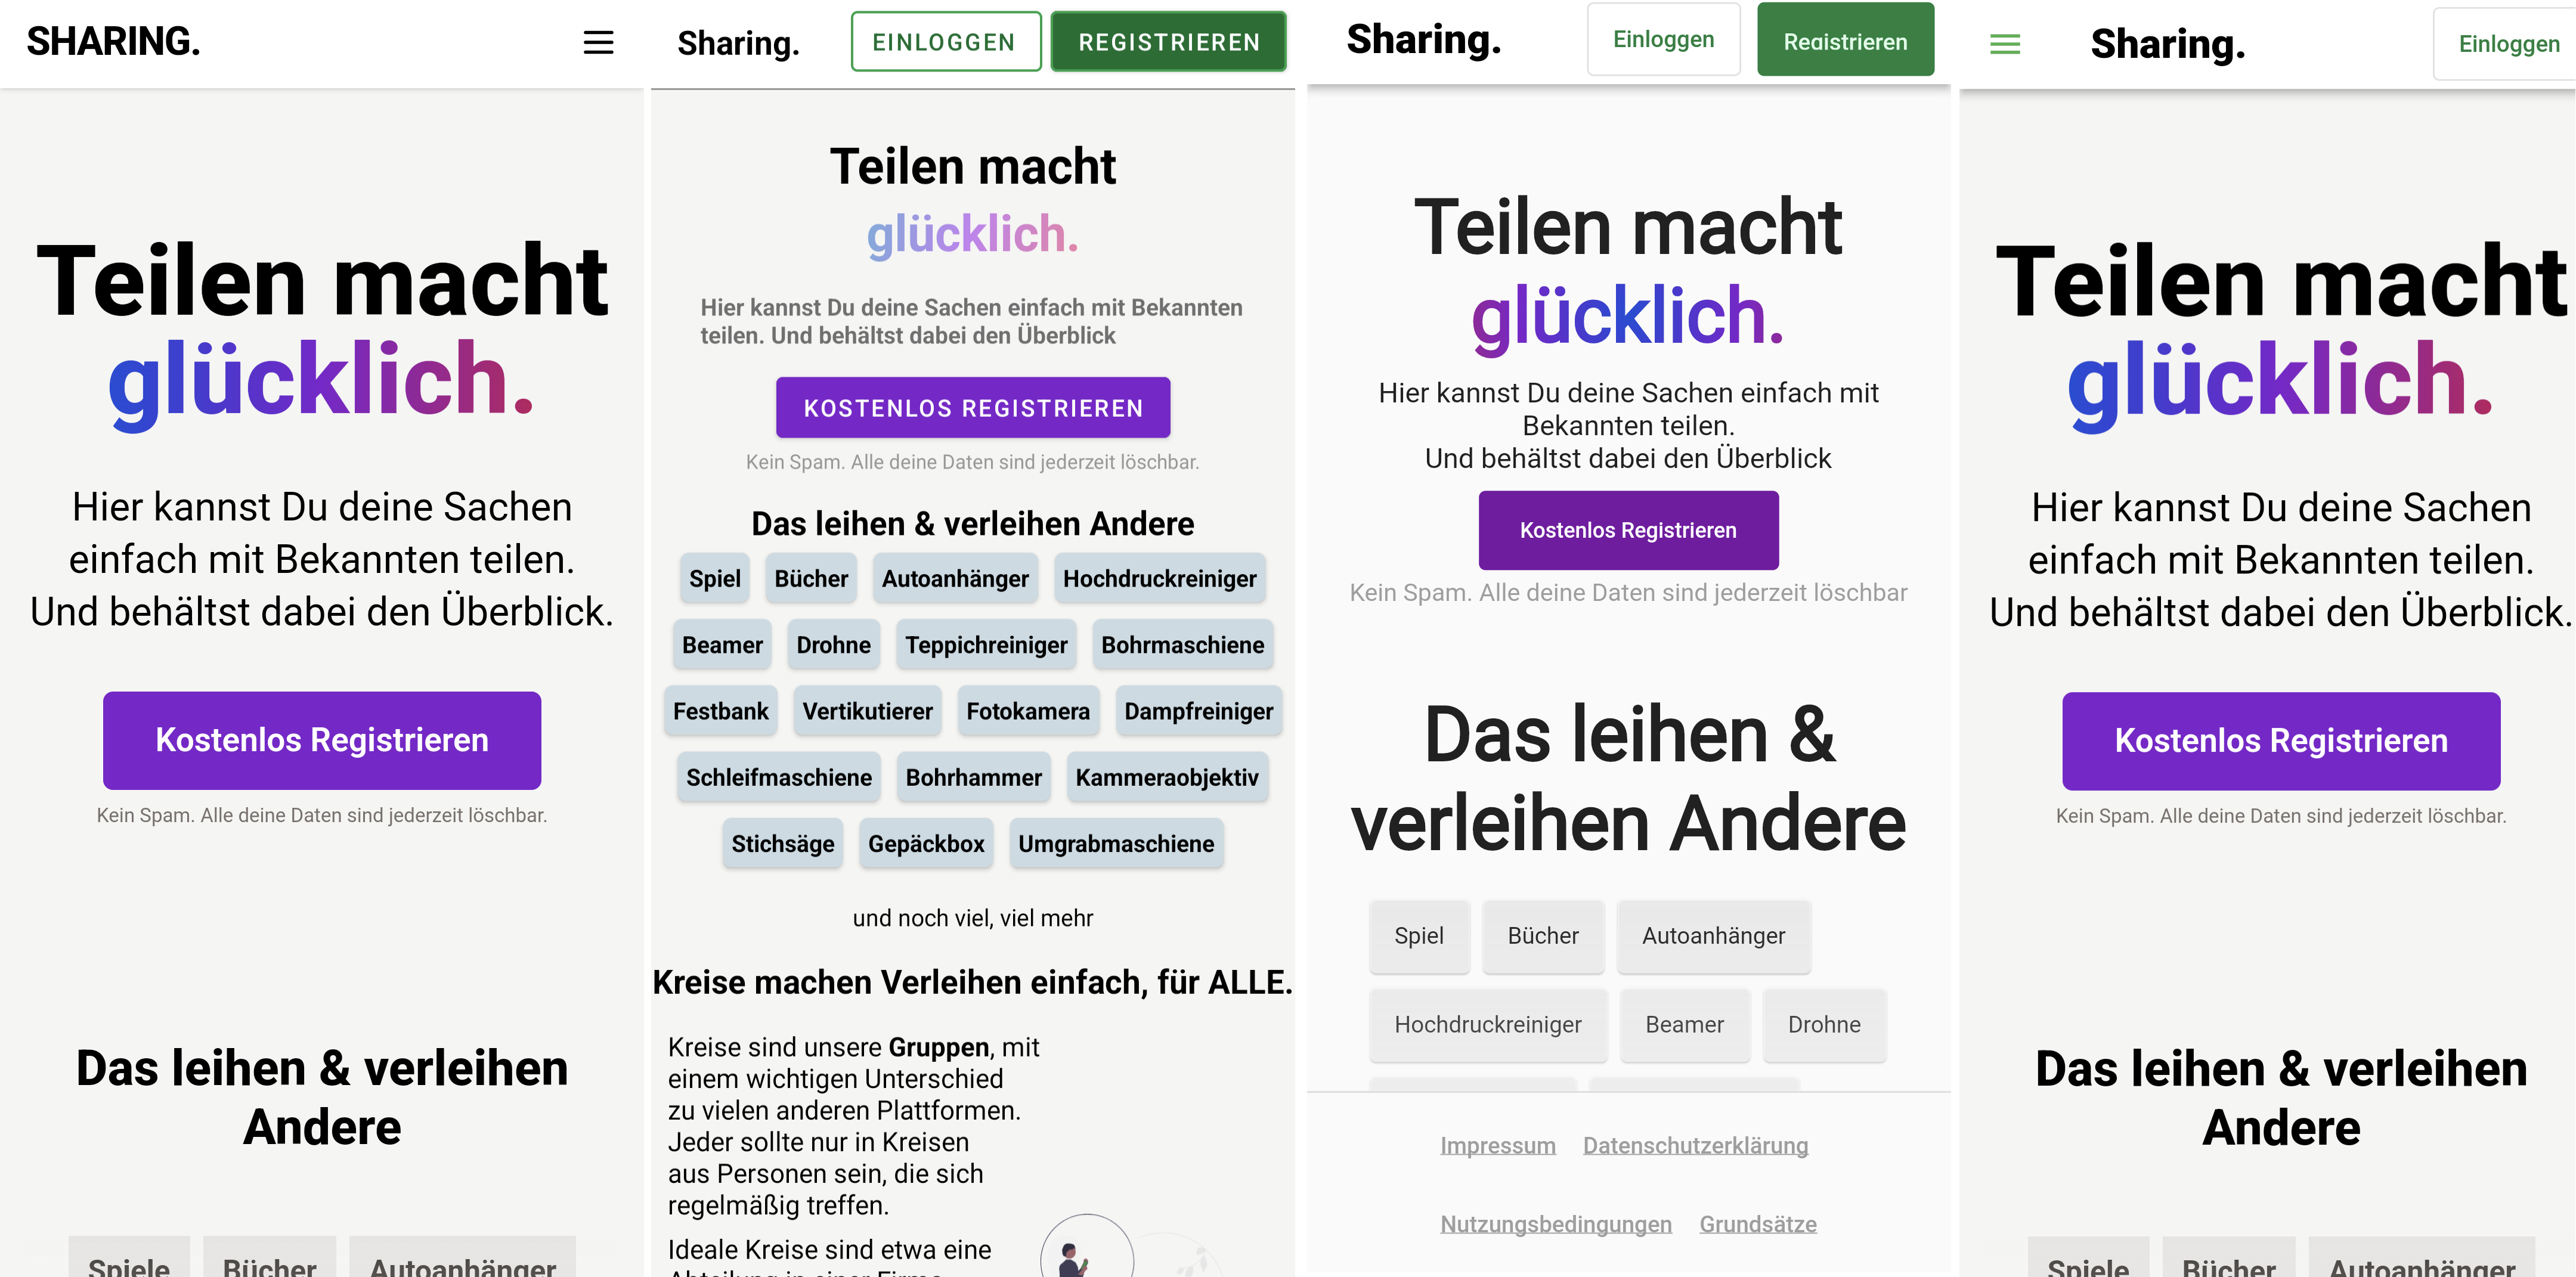
\includegraphics[height=7cm,keepaspectratio]{images/Startbildschirm_vergleich.png} 
  \caption[Vergleich des Startbildschirms der Implementierungen]{Vergleich des Startbildschirms der Implementierungen. Von links nach rechts: Hybride-Applikation, native Kotlin Applikation, Flutter Cross-Plattform-Applikation, Flutter Hybride Applikation}
  \label{fig:startscreen}
\end{figure}

In Abbildung \ref{fig:startscreen} sind die Startbildschirme der verschiedenen Anwendungen zu sehen. Für alle wurde eine etwa gleich lange Maximalzeit verwendet, um das Ergebnis vergleichen zu können. Der erste Bildschirm ist von der Webversion. Für diese wurde am wenigsten Zeit genutzt, da an ihr nicht viel geändert werden konnte. Sie ist also die gleiche Darstellung wie wenn die Webseite im Browser aufgerufen werden würde.  Sie ist, wie es auffällt bereits stark für mobile Geräte optimiert und sieht dementsprechend gut nutzbar aus. Was bei ihrer jedoch negativ auffällt, sind die nicht nativen Elemente durch die reine Nutzung von JavaScript.
So ist in Abbildung \ref{fig:sidemenu} die Seitenmenüanzeigen anhand von Flutter und durch die Webimplementierung gezeigt. Hier merkt man bei der Nutzung deutlich, dass die Web-Implementierung für PC Nutzer ausgelegt ist, mit dem Ziel gut für Smartphone Nutzer bedient zu werden, während die Flutter Implementierung deutlich besser für die Nutzung an einem Smartphone ausgelegt ist. Dies ist besonders gut spürbar, da das Menü der Webseite nur über einen Knopf und manuelles drücken nutzbar ist, während in der Flutter Implementierung von der Seite gewischt werden kann um die Vorteile eines Touchscreens auszunutzen.

\begin{figure}[ht]
  \centering
  \includegraphics[height=7cm,keepaspectratio]{images/Seitenmenü_vergleich.png} 
  \caption[Vergleich des Seitenmenüs bei nativer Implementierung und JavaScript Implementierung]{Vergleich des Seitenmenüs bei nativer Implementierung (links) und JavaScript Implementierung (rechts).}
  \label{fig:sidemenu}
\end{figure}

Während auf der Webseite einiges an Zeit und ein extra Designpakete genutzt wurden, um das insgesamte Aussehen der Anwendung zu verändern, wurde bei den getroffenen Implementierungen lediglich die Farben angepasst. Bei der Flutter Implementierung wirken die Elemente dabei deutlich moderner und angepasst für eine Smartphone-Applikation. Das wird besonders deutlich, wenn die Login-Screens verglichen werden.

\begin{figure}[ht]
  \centering
  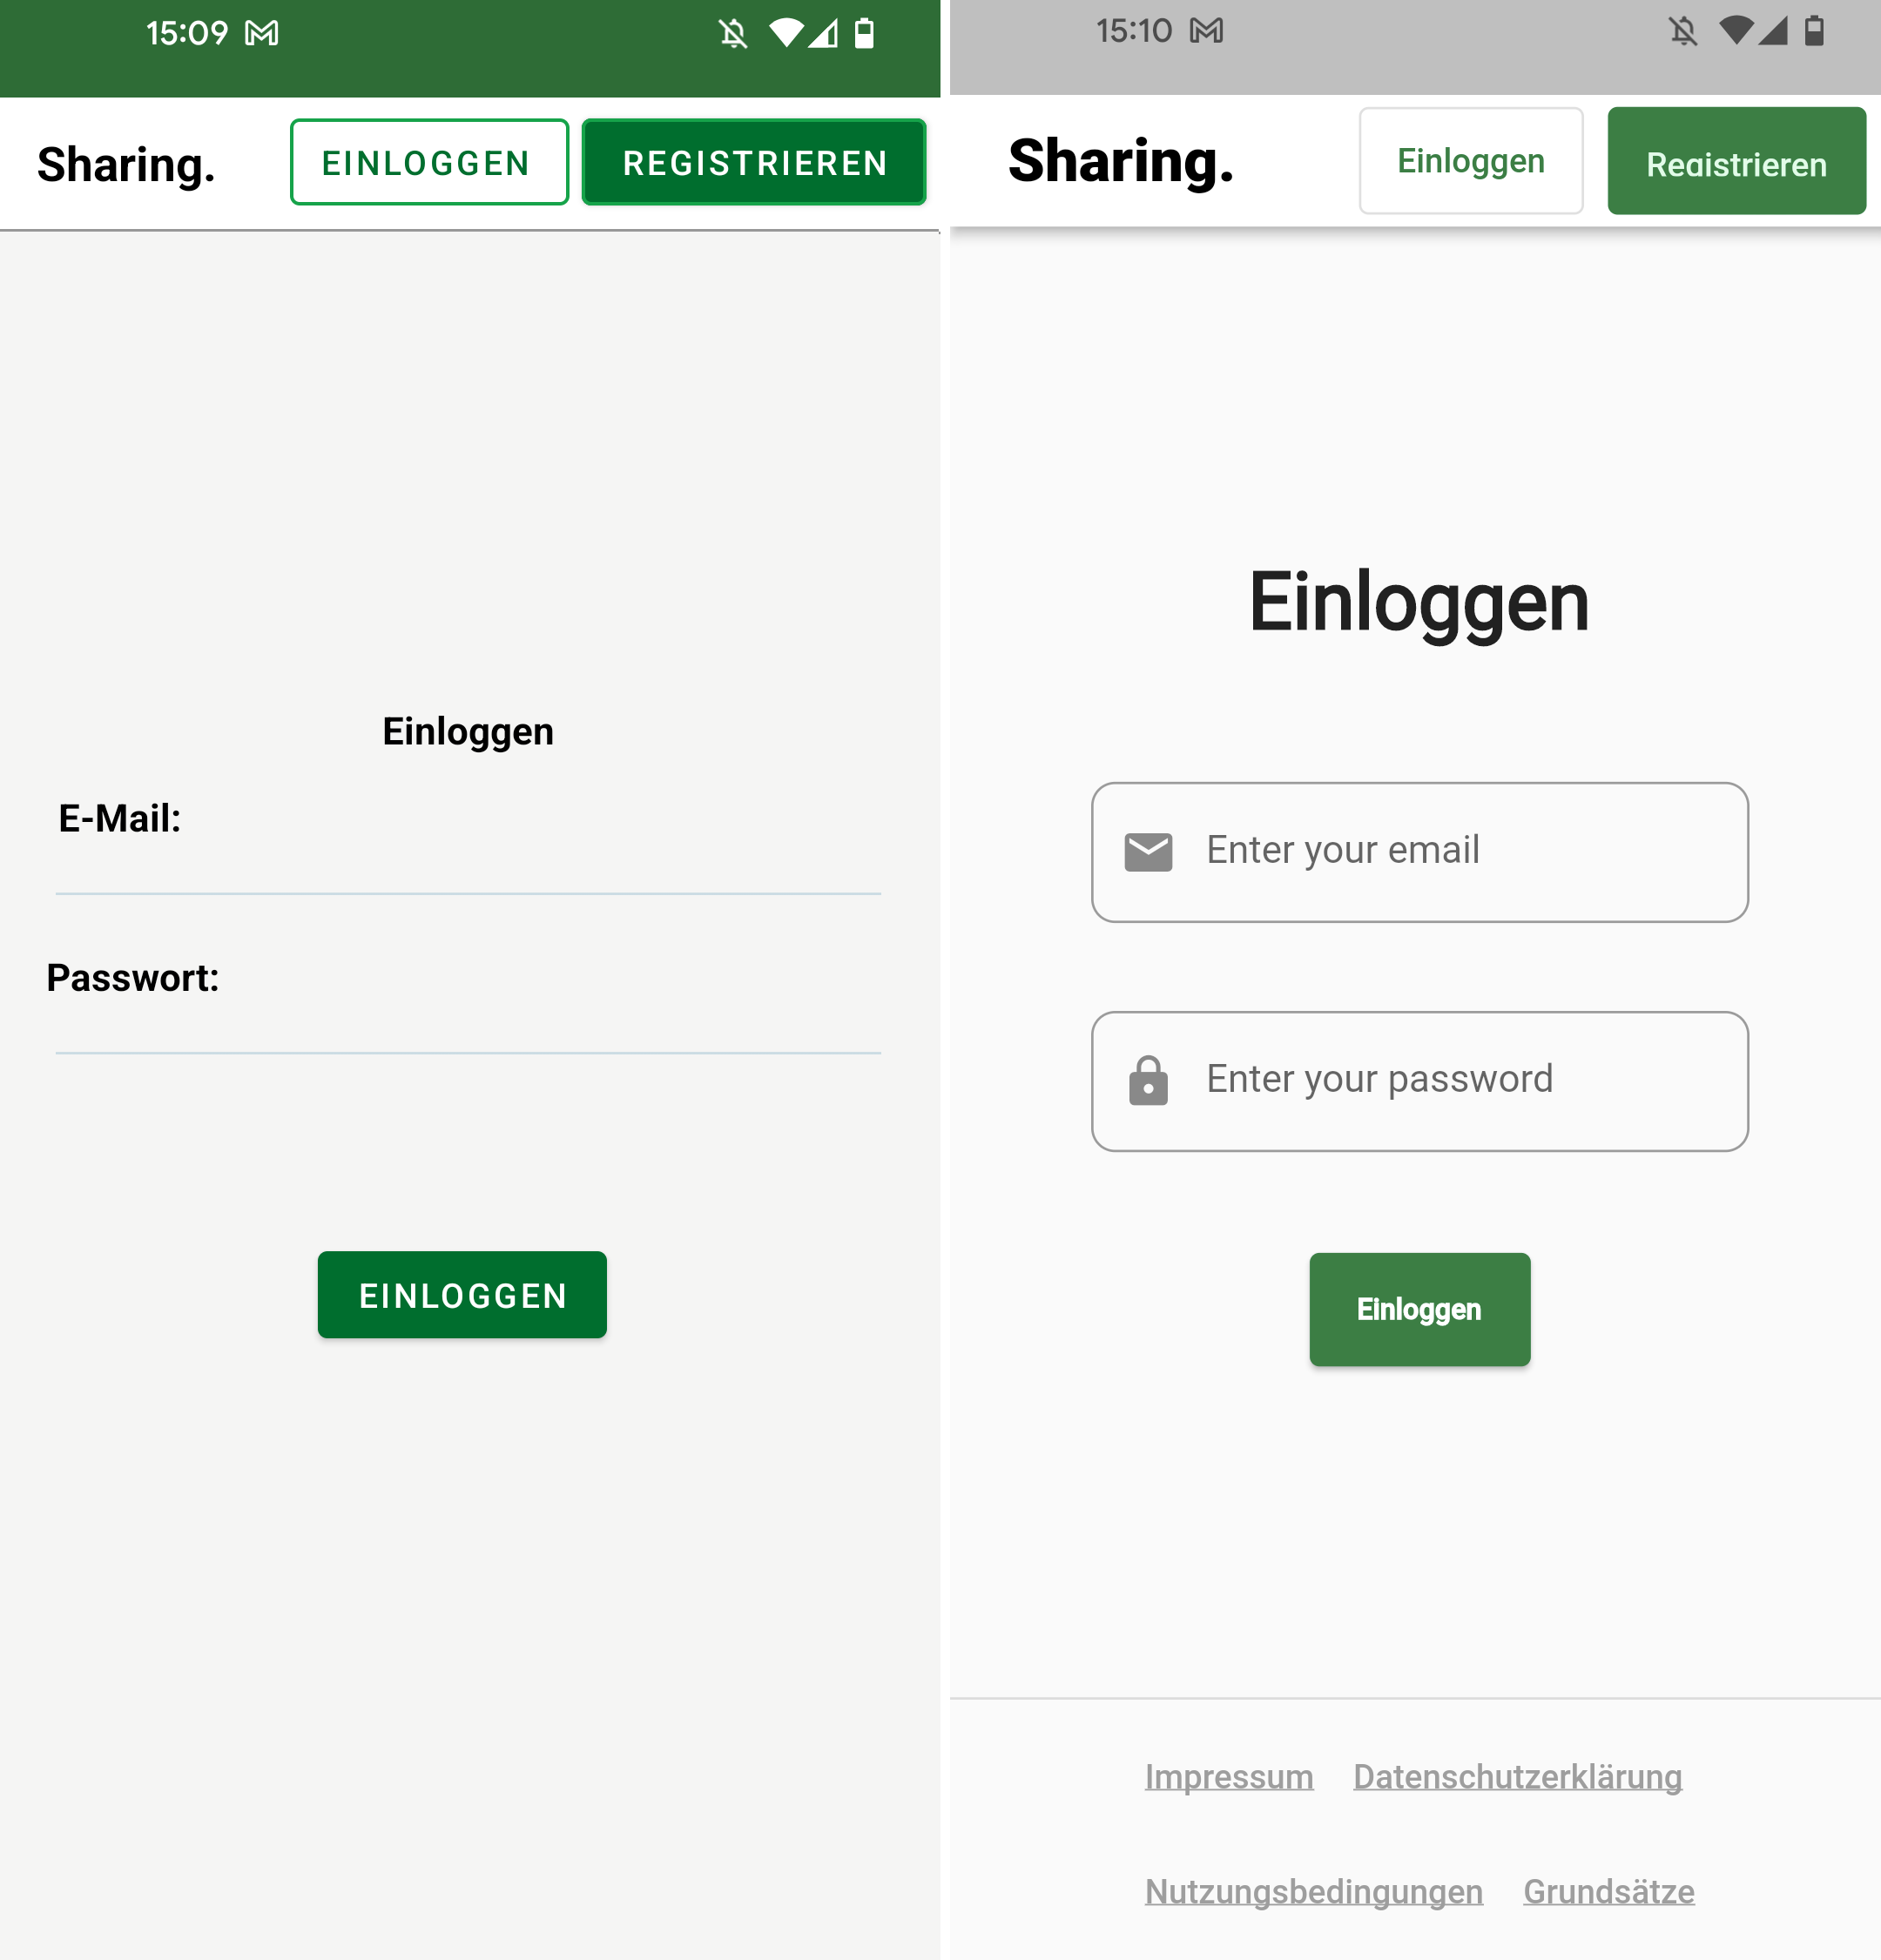
\includegraphics[height=7cm,keepaspectratio]{images/Login_vergleich.png} 
  \caption[Vergleich des Login-Bildschirms von Kotlin und Flutter Implementierung.]{Vergleich des Login-Bildschirms von Kotlin (links) und Flutter (rechts) Implementierung.}
  \label{fig:loginscreen}
\end{figure}

In Abbildung\ref{fig:loginscreen} ist der Loginscreen der nativen und des Cross-compilierten Ansatzes zu sehen. Wie bereits erwähnt hat Flutter ein deutlich besseres Out-of-the-Box Design Paket. Die Input Felder bei der Koltin Implementierung wirken dabei einfach veraltet und nicht dem Standard einer modernen App Entwicklung angepasst.

Das Aussehen der einzelnen Apps ist durch Erweiterungen und sonstiges stark anpassbar. Wie aber ersichtlich geworden ist, bietet Flutter die am modernsten und passend wirkende Standardkonfigutration für die Benutzeroberflächen. So ist die Entwicklung einer \ac{UI} in Flutter deutlich schneller und mit weniger Konfigurationsaufwand verbunden, als mit jeder anderen betrachteten Implementierung.

\subsubsection{Konsistenz über Plattformen hinweg}
Ein weiterer Aspekt bei der Entwicklung der Nutzeroberfläche ist die Konsistenz über Plattformen hinweg. Das Ziel ist es dabei, dass der Nutzer keinen Unterschied bemerkt, wenn er von einer Plattform zu einer anderen wechselt. 
Dies bedeutet, dass wo immer unterschiedliche Implementierungen für die Plattformen geschrieben werden, die Gefahr für Inkonsistenz am höchsten ist.
Dementsprechend sind Implementierungen die für mehrere Plattformen wieder verwendet werden können ein positiver Faktor um die Konsistenz zu fördern.
Auf die in dieser Arbeit vorgestellten Implementierungen bezogen, bedeutet dies, dass die reine native Implementierung eine höhere Gefahr von Inkonsistenz besitzt, als etwa die hybride oder Flutter Applikation.
Dabei ist allerdings zu erwähnen, dass auch die nativen Applikationen einen hohen Grad an Konsistenz erreichen können. Dies bedeutet jedoch häufig einen höheren Aufwand bei der Implementierung und eine enge Zusammenarbeit der Entwickler der verschiedenen Plattformen.

\subsubsection{Plattformabdeckung \& Wiederverwendbarkeit}
Wie an mehreren Stellen der Arbeit bereits erwähnt sind nativ entwickelte Applikationen immer nur für eine Plattform entwickelt. Sie haben dementsprechend auch den am wenigsten wiederverwendbaren Code, da lediglich die Logik geteilt werden kann, jedoch die genaue Implementierung für jede Plattform unterschiedlich ist. Jedoch kann für jede Plattform eine native Apllikation geschrieben werden.

Hybride Apps haben hier bereits einen deutlich höheren Wiederverwenbarkeitsgrad, da bei ihnen ja lediglich die Anzeigelogik ausgetauscht werden muss, aber die iegentliche Implementierung in einer Webtechnologie getan wurde, wodurch sie auf fast jeden Gerät genutzt werden kann. Jedoch können einige Technologien auf ein paar Plattformen beschränkt sein. Desweiteren kann es bei dieser Klasse durchaus Probleme geben, wenn sie zu einem großen Anteil aus der Ansicht der Webseite besteht. So wurde ja bereits die Richtlinien von Apple erwähnt, die diese Klasse zu einem gewissen Grad aus dem App-Store verbannt. Da hybride Applikationen außerdem einen nativen Code-Teil besitzen, sind sie wieder nur auf einer Plattform installierbar. 

Cross-Plattform-Applikationen werden mit einer Technologie gebaut, um mehr als eine Plattform mit einem Code abzudecken. Dabei ist dies zwar von der genau genutzten Technologie abhängig, aber in dem vorgestellten Fall sind 5 Plattformen damit abdeckbar. Mit Flutter und der Wahl der richtigen Erweiterungen sind nach aktuellem Stand sogar 6 Plattformen möglich. Außerdem kann durch die Wahl von Flutter der gleiche Code für alle Plattformen genutzt werden. Eine Wiederverwendbarkeit ist so gesehen also nicht bewertbar, da es theoretisch nicht nötig ist den Code für eine andere Implementierung wiederzuverwenden. Wenn allerdings der Code für eine andere Implementierung genutzt werden sollte ist es wie im nativen Fall, dass nur die Applikationslogik nutzbar ist, da die Anwendung in ihrer eigenen Programmiersprache geschrieben ist.

Die Flutter-Web Implementierung ist in diesem Aspekt ähnlich zu der Flutter Implementierung. So gelten grundsätzlich die gleichen Aussagen, jedoch mit Einschränkung der Anzahl der abgedeckten mobilen Endgeräte. So ist diese Implementierung lediglich auf den beiden Plattformen Android und iOS nutzbar. Wie bereits erwähnt ist dies Abhängig von der Web-Container Implementierung und kann mit der Wahl eines passenderen Containers oder Eigenentwicklung eines eigenen Browser-Plugins auf die restlichen Plattformen erweitert werden.

\subsubsection{Programmieraufwand}
Der genaue Programmieraufwand ist immer stark abhängig von den genauen Vorkenntnissen, der genutzten Technologie und externen Bibliotheken und natürlich dem Umfang der Anwendung. Ein Anhaltspunkt sind die \ac{LOC} die für die einzelnen Implementierungen geschrieben wurden, um dies ein wenig vergleichen zu können. Dafür wurden die einzelnen Daten mit Hilfe des Statistics\footnote{https://plugins.jetbrains.com/plugin/4509-statistic} Plug in gesammelt. Dabei wurden die gesammelten Daten in die drei Typen Konfiguration, Oberfläche/UI und Logik unterteilt. Bei den zwei Implementierungen die außerdem noch Teile der Webseite mit anzeigen, wurden außerdem die in der Anwendung abgedeckten Programmteile erfasst, da diese für eine Implementierung auf dem Stand genauso notwendig ist. Zusätzlich wurde der benötigte Code untersucht um die Liste der Gegenstände anzuzeigen. Also sowohl die Layoutdatein, als auch die benötigte Anwendungslogik.\TODO{Weiß nicht ob Logik hier der richtige Begriff ist, da dies ja auch das hinzufügen der Oberflächenfunktionalität ist.}
Bei den Implementierungen, bei denen Flutter genutzt wurde, ist die Oberflächen und Logikcode Zeile zusammengefasst, da dies bei Flutter in einer Datei geschrieben wird. 

\begin{table}
\centering
\caption{Programmlänge der verschiedenen Implementierungen in \ac{LOC}}
\begin{tabular}{ |p{4.5cm}||p{3cm}|p{2cm}|p{2cm}|p{3cm}|p{3cm}| }
 \hline
 Programmteile in Lines of Code & Flutter-Web & Flutter & Kotlin-Nativ & Kotlin-Hybrid \\
 \hline
 Gesamte Anwendung       &   2391(App) + 2033(Web) &   2100 & 3138 & 449(App) + 2814(Web)\\
  \hline
 Konfigurationscode  & 42 + 268& 32& 229& 16 + 357\\
  \hline
 Oberflächencode &\multirow{2}{*}{2349 + 1765}  &\multirow{2}{*}{2068}  & 1958& 334 + 1768\\
  \cline{1-1}
  \cline{4 -5}
 Logikcode & & & 951& 99 + 689\\
  \hline
 Beispeil: Liste an Gegenständen & 65 & 65 & 178 & 71(Web)\\
  \hline
\end{tabular}
\label{tab:lines_of_code}
\end{table}

In Tabelle \ref{tab:lines_of_code} sind die \ac{LOC}s der einzelnen Implementierungen auf verschiedenen Programmteile aufgeschlüsselt zu sehen. Dabei wurde auch der Code der genutzten WebImplementierung dazugerechnet, da diese ein Teil der jeweiligen Anwendung ist. Die wenigsten Zeilen hat die reine Flutter Implementierung und die meisten die Flutter-Web Implementierung.  Die Flutter-Web Implementierung besteht dabei in etwa zu einer Hälfte aus der Flutter Implementierung und zu einer Hälfte aus der Web Implementierung. Die hybride Implementierung hat zwar den wenigsten Code für die Applikation an sich, hat jedoch durch die Webseitenimplementierung mehr Zeilen als die native Applikation, jedoch weniger als die Flutter-Web Implementierung. 

Bei dem untersuchten Beispiel einer Liste für Gegenstände ist wieder die Flutter Implementierung die mit dem geringsten Code. Dabei entfallen 55 Zeilen auf die Anzeige eines Gegenstandes und gerade einmal 10 Zeilen Code um die Liste einzubauen und zu konfigurieren. Ähnlich ist dies bei der Webseite. Einzig die native Kotlin App hat hier ein erhöhten Aufwand. Dabei entfallen 75 Zeilen auf das Design und weitere 83 Zeilen auf die Steuerung der Liste und dem hinzufügen der Daten. Ein Großteil davon ist der Adapter der benötigt wird um die Liste zu steuern. Durch solche Konstrukte benötigt Kotlin mehr \ac{LOC}, als etwa die Flutter Implementierung.

Bei den Implementierungen in der die Webseite eingebaut sind, fügt die Webseite einen hohen Teil der Zeilen hinzu. Dies ist aber zu einem gewissen Teil dem Aufbau des Webcodes geschuldet. So ist bei dem Vergleich des benötigten Codes für die Liste, die Webseite gerade mal 6 Zeilen hinter der Flutter Implementierung und damit immer noch gerade mal halb so viel wie die Kotlin Entwicklung benötigt.

\subsubsection{Zeit bis zum Release}
Durch den Programmieraufwand und der Anzahl der zu unterstützenden Plattformen wird die Dauer der Entwicklungszeit und die Zeit bis zu einem möglichen Release stark beeinflusst. Genaue Werte sind dabei auch stark von Funktionsumfang, Anzahl der Entwickler und den Vorraussetzungen abhängig. Jedoch lassen sich dennoch einige Aussagen treffen.

So ist etwa ein Release der Nativen Anwendung am aufwendigsten. Nicht nur dass wie bereits gesehen, mit der meiste Code geschrieben werden muss, muss dies auch noch für jede Plattform passieren. Am schnellsten ist dies bei der Cross-Plattform Implementierung mit Flutter. Hier muss lediglich einmal die Anwendung durchprogrammiert werden und kann im Anschluss für die einzelnen Plattformen einfach nur noch exportiert werden. Nach der reinen Flutter Implementierung ist die Flutter Implementierung mit Webanteil. Diese ist dann gefolgt vom hybriden Ansatz. 

Wenn jedoch die Webseite bereits existiert und dementsprechend nicht bei der Implementierzeit beachtet werden muss, ändert sich hier die Reihenfolge sehr wahscheinlich je nach umfänglichkeit der Zusatz Implementierung des Flutter Web Ansatzes.

Der Flutter-Web Mixansatz kann außerdem noch von hohem Vorteil sein, wenn eine Webseite in eine App verwandelt werden soll. Denn hier kann wie bei der hybriden Implementierung eine anfängliche Version veröffentlicht werden, die lediglich die Webseite öffnet und danach Stück für Stück die Webseite durch Flutter Seiten ersetzen. So kann der Nutzer jederzeit die komplette Anwendung nutzen und bekommt Stück für Stück eine angepasste Appversion.

\subsubsection{Offline Funktionalität}
Es gibt einige Fälle in denen der Nutzer unter Umständen eine Applikation weiter nutzen will, auch wenn er aktuell keine aktive Internetverbindung hat. In diesem Fall benötigt die Applikation eine offline Funktionalität.

Wie bereits an mehreren Stellen in dieser Arbeit erwähnt haben die Implementierungen, die die Webseite als Teil ihrer Implementierung haben, hier oft keine Funktionalität. Im Falle der Flutter-Web Applikation kann die Funktionalität zumindest teilweise erreicht werden, indem andere Seiten angezeigt werden die nativ implementiert werden. Die native und Cross-Compilierte Lösung haben hier eindeutig den besseren Standpunkt. Ihre Anzeige ist unabhängig von einer aktiven Internetverbindung nutzbar. Hier kommt es lediglich darauf an, ob die Daten, die in der App angezeigt werden auf dem Gerät gespeichert werden oder ob sie immer von einem Server abgefragt werden müssen. 

Hier ist allerdings zu erwähnen, dass andere hybride Ansätze zwar auch Webtechnologie nutzen, jedoch die Daten alle lokal auf dem Gerät gespeichert werden. In diesem Fall hätte auch der hybride Ansatz offline funktionieren. Der in diese Arbeit gewählte Ansatz jedoch nicht.


\subsubsection{Lesbarkeit und Übersichtlichkeit der Implementierung}
Bei der Übersichtlichkeit ist es wieder eine Frage nach der Art der Implementierung. 

\section{Fragekompass um eine Auswahl zu treffen}
1. Existiert bereits eine Webseite, die in eine App umgewandelt werden soll?
    Wenn eine Webseite bereits existiert, sind der hybride und der Web-Flutter Ansatz eine gute Option. Denn durch die Integration kann sowohl ein großer Teil der Implementierung vermieden werden, selbst wenn letztlich nicht die Webseite in der App angezeigt wird, sondern die echten HTML Datein. Denn diese können im Zweifelsfall kopiert und falls benötigt umgearbeitet werden.
    
    Es kann einen fließenden Übergang von Webseite zu komplett Implementierter Applikation geben soll. So kann bei dem entwickelten gemixten Ansatz eine erste Version schnell entwickelt werden, die ausschließlich aus der Webseite besteht und dann Stück f
2. Ist Performance Priorität Nummer 1 ?

3. Sollen mehr als nur eine Plattform abgedeckt werden ?

4. Existiert bereits eine Applikation die nur etwas geändert werden soll?

5. 

